%!TEX root=report.tex
\subsection{Kernel PCA}

Before delving into kernel methods, the standard PCA method will briefly be recapped.
PCA as introduced in this report was done via SVD ($X = U\Sigma V^T$). The columns of $U$ is the eigenvectors of $XX^T$. The projected space is then $Z = XV = U\Sigma$. 
Looking at the dependencies of $U$, it is apparent that the principal component scores, will end up being linear combinations of basis in original input space $X$. 
In most cases this suffices but what if there are no linear relationships in the $X$ space, standard PCA won't be appropriate.

\subsubsection{Motivating example}
\begin{figure}[H]
	\center
	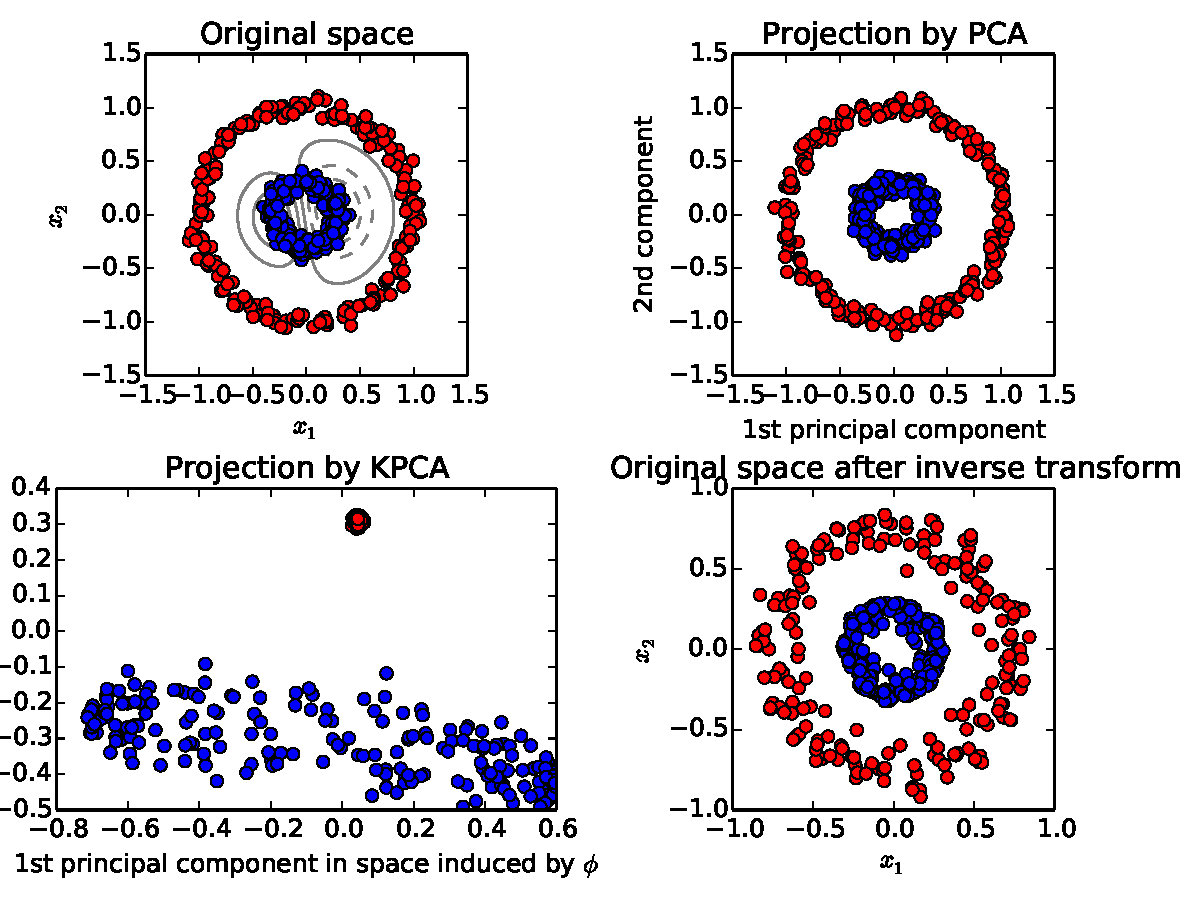
\includegraphics[width=\textwidth]{figures/kernel-pca-example}
	\caption{Motivating kernel PCA example. Image courtesy of scikit-learn. License: BSD 3 clause. Authors: Mathieu Blondel and Andreas Mueller.}
	\label{fig:kernel-pca-example}
\end{figure}

As is seen in Figure \ref{fig:kernel-pca-example}, classes that wasn't linearly separable in the original space can be become linearly separable in the kernel space. This in turn makes clustering much easier and hopefully improves results.

\subsubsection{The Kernel Trick}

In kernel PCA, instead of working on $X X^T$, a nonlinear mapping $\Phi: X\rightarrow Y$ is used, such that the SVD is carried out on $\Phi(X)\Phi(X)^T = K(X, X^T)$. Specifically one define the inner product as a function of $(x_i, x_j)$, thus $\Phi(X)\Phi(X)^T$ is calculated, but without the need for the nonlinear mapping function $\Phi$. This inner product function is the kernel.
 
For something to be a valid kernel, all the kernel needs to satisfy is to be function of an inner product in some vector space.
For the above to become more clear, let us give an example of a polynomial kernel in a 2-dimensional space. in the following $X$ is a vector and $X'$ is simply some other vector in the same space as $X$:
\begin{equation}
\begin{split}
K(X,X') &= (1+X^T X')^2 = (1+x_1 x'_1+x_2 x'_2)^2 \\
&= 1+x_1^2 {x'}_1^2 +2 x_1 x'_1 + 2 x_2 x'_2 + 2 x_1 x'_1 x_2 x'_2
\end{split}
\end{equation}

For the above to actually be a actual kernel there would have to be some transformed space in which the above was an inner product. From the coefficients above it can be deduced that the basis in this transformed space must be given as
\begin{equation}
(1,x_1^2,x_2^2,\sqrt{2} x_1, \sqrt{2} x_2 , \sqrt{2} x_1 x_2)
\end{equation}

Now consider if one used a power of 100 instead of 2. Calculating the kernel in the non transformed  space is easy; $(1+X^T X')$ is just a number and raising it to the power of 100 can be done quickly.
On the other hand if one were to explicitly calculate the kernel as the inner product in the transformed space, a huge vector would have to be computed, transposed and be subjected to an the inner product in this space. This is clearly not very efficient.

The shortcut to define $K$ instead of $\Phi$ is called the Kernel Trick.

\subsubsection{The Radial Basis Function (RBF) kernel}

The RBF kernel is commonly used when the amount of samples is much larger than the amount of dimensions in the original space.

The RBF kernel is defined as
\begin{equation}
K(x,x')=\mathrm{exp}(-\gamma ||x-x'||^p_2)
\end{equation}

The above can easily be calculated. The following shows that the above is indeed an inner product. It is not a complete proof as $\gamma=1, p=2$ and $x$ is a scalar not a vector.

\begin{equation}
\begin{split}
	K(x,x')&=\mathrm{exp}(- ||x-x'||^2_2)=\mathrm{exp}(- (x-x')^2) \\
		  &= \mathrm{exp}(-x^2) \mathrm{exp}(-{x'}^2) \mathrm{exp}(2 x x')
\end{split}
\end{equation}
since $\mathrm{exp}(2 x x')$ can be Taylor expanded to $\sum_{k=0}^\infty \frac{2^k(x)^k (x')^k}{k!}$ it follows that:
\begin{equation}
K(x,x') = \sum_{k=0}^\infty \left(\sqrt{\frac{2^k}{k!}} (x)^k \mathrm{exp}(-x^2)\right)\left(\sqrt{\frac{2^k}{k!}} (x')^k \mathrm{exp}(-{x'}^2)\right)
\end{equation}

From the above it is seen that for any k, the term in the right parenthesis is exactly equal to the left parenthesis, if $x'$ was substituted with $x$. This means that in an expanded vector space, this correspond to the the inner product from the $\ell^2$ Hilbert space. Do also note that since the sum is infinite, the transformed vector space is of infinite dimensional space and is thus impossible to calculate without the kernel trick.

\subsubsection{Mercer's Condition}
Proving that something is a kernel, is actually easier than shown above. It is done using Mercer's Condition, though it dose not say anything about the size of the space when $\Phi$ is applied.

The theorem says, that given all real valued square integrable functions $g$ (${g \in \{\mathbb{R} \rightarrow \mathbb{R}\} \cap L^2(\mathbb{R})}$). That is the following must be true:
\begin{equation}
\int_{-\infty}^{\infty} g(x)^2 \mathrm{d}x < \infty
\end{equation}

Then for all these $g$ functions, if the following condition holds:
\begin{equation}
\int \int K(x, y) g(x) g(y) \mathrm{d}x \mathrm{d}y \ge 0
\end{equation}

Then $K$ is a valid kernel.

\subsubsection{Final notes of kernel PCA}

In kernel PCA the columns of $U$ is the eigenvectors of $K(X,X^T)$ and the columns of $V$ the eigenvectors of $K(X^T,X)$. The size of $X X^T$ and $X^T X$ is going to be $nxn$ and $pxp$ respectively where $n$ is the number of samples and $p$ the dimensions in transformed space. Thus when dealing with kernel PCA the calculation of $V$ is omitted and calculation of $U$ is expensive, but possible.

In the case of the GRACE data the size of $X$ is ($64800 \times 341$). Memory wise this results in a $U$ matrix of size ($64800 \times 64800$) with float32 numbers, that is approximately $15.64\text{ GB}$. Furthermore kernel PCA also involves quite a lot of simple computing. So for practical purposes one should use a computer cluster (e.q. the DTU HPC cluster).
